%%%% Ecriture du plan

\section*{Introduction}

\section{Etat de l'art}

\subsection{Problématiques et historique}

% idée : d'où ça sort ce concept de gestionnaire de versions ?
% Quels problèmes ont été résolus par les gestionnaires de versions, comment/quels sont les différentes solutions? 

\subsubsection{Mauvaises pratiques}

Au commencement était l'information. Et l'information était à gérer, et l'information posa problème. Les développeurs de logiciels qui travaillaient en équipe devaient se soucier de mettre en commun leurs modifications. 
Nous étions à la préhistoire de l'informatique.
% (ère qui n'est peut-être pas révolue de nos jours, comme nous verrons par la suite)

Plusieurs solutions furent envisagées, des plus téméraires aux plus banales:
\begin{itemize}
\item CPOLD : pour mettre en commun une modification, nous gardions une copie du fichier d'origine, renommé en \texttt{.old} et nous copions le nouveau fichier sur un répertoire commun ~\cite{CPOLD-article}. 
\item La solution de la disquette : chaque modification pouvait être transmise par un nouveau fichier via une disquette, un e-mail ou autre.
\item De nos jours encore, certaines personnes utilisent un service de synchronisation dans le cloud (du type Dropbox/SugarSync) pour synchroniser leurs fichiers et dossiers sur tous les ordinateurs. 
\end{itemize}

Ces façons de gérer les ressources présentaient de nombreux défauts. Nous pouvons noter en particulier : 
\begin{enumerate}
\item le manque de robustesse et la perte de données possibles en cas d'erreur lors de la copie ;
\item l'impossibilité de remonter aux anciennes versions des fichiers ;
\item la redondance de l'information. Une grande partie des modifications n'affecte pas l'ensemble du fichier ;
\item le manque d'automatisation. Les opérations étaient réalisées à la main -- ou au mieux à l'aide de scripts bash, MDR! 
\end{enumerate}

\subsubsection{L'invention du gestionnaire de versions}

Nous sommes dans les années 80, l'essor du logiciel libre attire de plus en plus de développeurs. 
Ceux-ci collaborent sur des projets dont la complexité s'accroît au cours du temps. 
La gestion de projets d'une telle envergure nécessite des outils adaptés. 
Afin de répondre aux problématiques sus-citées, ils ont développé plusieurs solutions. 

La première solution stable sortit dans le cadre du projet GNU, initié par Richard Stallman. Il s'agit de RCS (acronyme pour Revision Control System) ~\cite{GNUWebSite}. 
Celui-ci est une amélioration de SCCS (Source Code Control System). Il présente une interface plus simple d'utilisation, un stockage amélioré des versions de fichiers afin de les retrouver plus rapidement. 

\subsubsection{Généalogie}

Puis ils se marièrent et eurent beaucoup d'enfants. L'arbre donné en figure \ref{fig:chronologie} retrace leur généalogie. 


\begin{figure}[h!]
  \centerline{
  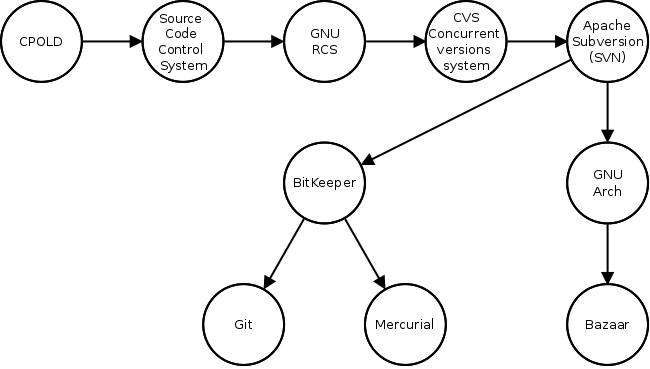
\includegraphics[width=14cm]{images/chronologie.png}}
  \caption{Résumé des gestionnaires de versions à travers l'histoire}
  \label{fig:chronologie}
\end{figure}

RCS engendra CVS. CVS engendra SVN. SVN fut fécond et insuffla la vie à deux enfants, BitKeeper et GNU Arch. 
A ce moment, deux ramifications se produisirent dans la descendance. 

\subsection{Cahier des charges d'un gestionnaire de versions}

% idée : c'est quoi un gestionnaire de versions ?
% et qu'est-ce qui les distingue?

% On récapitule toutes les fonctionnalités clés : branches, commit, merge, stage, repo, centralisé, décentralisé, diff

\subsection{Récapitulatif/Comparatif des gestionnaires de versions}

% idée : quels sont les différents gestionnaires de versions ? Qu'est-ce qui les différencie ? 
% & Comment sont-ils apparus ?
% - bitkeeper, git
% - cvs, svn

\section{Etude de GIT}

\subsection{Choix de GIT}

\subsection{Utilisation de GIT}

\subsection{Détails sur le fonctionnement de GIT}

\section*{Conclusion}



%%% Local Variables: 
%%% mode: latex
%%% TeX-master: "rapport_master"
%%% End: 
